% !TEX TS-program = xelatex
% !BIB program = bibtex
% !TeX spellcheck = ru_RU

% About magic macros see also
% https://tex.stackexchange.com/questions/78101/

% По умолчанию используется шрифт 14 размера.
% Если Вы не влезаете в лимит страниц и нужен 12-й шрифт,
% то уберите опцию [14pt]
\documentclass[14pt, russian]{matmex-diploma-custom}

% !TeX spellcheck = ru_RU
% !TEX root = burashnikov_depinspect.tex
% Опциональные добавления используемых пакетов. Вполне может быть, что они вам не понадобятся, но в шаблоне приведены примеры их использования.
\usepackage{tikz} % Мощный пакет для создание рисунков, однако может очень сильно замедлять компиляцию
\usetikzlibrary{decorations.pathreplacing,calc,shapes,positioning,tikzmark}
\usepackage{pifont}
% Библиотека для TikZ, которая генерирует отдельные файлы для каждого рисунка
% Позволяет ускорить компиляцию, однако имеет свои ограничения
% Например, ломает пример выделения кода в листинге из шаблона
% \usetikzlibrary{external}
% \tikzexternalize[prefix=figures/]

\newcounter{tmkcount}

\tikzset{
	use tikzmark/.style={
			remember picture,
			overlay,
			execute at end picture={
					\stepcounter{tmkcount}
				},
		},
	tikzmark suffix={-\thetmkcount}
}

\usepackage{booktabs} % Пакет для верстки "более книжных" таблиц, вполне годится для оформления результатов
% В шаблоне есть команда \multirowcell, которой нужен этот пакет.
\usepackage{multirow}
\usepackage{siunitx} % для таблиц с единицами измерений

\newcommand{\cd}[1]{\texttt{#1}}
\newcommand{\inbr}[1]{\left<#1\right>}

% Для названий стоит использовать \textsc{}
\newcommand{\OCaml}{\textsc{OCaml}}
\newcommand{\miniKanren}{\textsc{miniKanren}}
\newcommand{\BibTeX}{\textsc{BibTeX}}
\newcommand{\vsharp}{\textsc{V$\sharp$}}
\newcommand{\fsharp}{\textsc{F$\sharp$}}
\newcommand{\csharp}{\textsc{C$\sharp$}}
\newcommand{\GitHub}{\textsc{GitHub}}
\newcommand{\SMT}{\textsc{SMT}}
\newcommand{\python}{\textsc{Python}}
\newcommand{\linux}{\textsc{Linux}}
\newcommand{\centos}{\textsc{CentOS}}
\newcommand{\ubuntu}{\textsc{Ubuntu}}
\newcommand{\debian}{\textsc{Debian}}
\newcommand{\fedora}{\textsc{Fedora}}

\newcolumntype{L}[1]{>{\raggedright\let\newline\\\arraybackslash\hspace{0pt}}m{#1}}
%\newcolumntype{C}[1]{>{\centering\let\newline\\\arraybackslash\hspace{0pt}}m{#1}}
\newcolumntype{R}[1]{>{\raggedleft\let\newline\\\arraybackslash\hspace{0pt}}m{#1}}

%  Команды и пакеты, не используемые в шаблоне, которые тем не менее могут быть полезными.

% \newcolumntype{Y}{>{\centering\arraybackslash}X}

% \usepackage{mathrsfs}

% \lstdefinelanguage{ocaml}{
% keywords={@type, function, fun, let, in, match, with, when, class, type,
% nonrec, object, method, of, rec, repeat, until, while, not, do, done, as, val, inherit, and,
% new, module, sig, deriving, datatype, struct, if, then, else, open, private, virtual, include, success, failure,
% lazy, assert, true, false, end},
% sensitive=true,
% commentstyle=\small\itshape\ttfamily,
% keywordstyle=\ttfamily\bfseries, %\underbar,
% identifierstyle=\ttfamily,
% basewidth={0.5em,0.5em},
% columns=fixed,
% fontadjust=true,
% literate={->}{{$\to$}}3 {===}{{$\equiv$}}1 {=/=}{{$\not\equiv$}}1 {|>}{{$\triangleright$}}3 {\\/}{{$\vee$}}2 {/\\}{{$\wedge$}}2 {>=}{{$\ge$}}1 {<=}{{$\le$}} 1,
% morecomment=[s]{(*}{*)}
% }


\begin{document}
% TODO: Formatting
% !TeX spellcheck = ru_RU
% !TEX root = artem-burashnikov_imageProcessingOnGPU.tex

%% Если что-то забыли, при компиляции будут ошибки Undefined control sequence \my@title@<что забыли>@ru
%% Если англоязычная титульная страница не нужна, то ее можно просто удалить.
\filltitle{ru}{
    %% Актуально только для курсовых/практик. ВКР защищаются не на кафедре а в ГЭК по направлению,
    %%   и к моменту защиты вы будете уже не в группе.
    chair              = {Кафедра системного программирования},
    group              = {ТП.22Б07-мм},
    %
    %% Макрос filltitle ненавидит пустые строки, поэтому обязателен хотя бы символ комментария на строке
    %% Актуально всем.
    title              = {Экспериментальное исследование обработки изображений с использованием GPGU},
    %
    %% Здесь указывается тип работы. Возможные значения:
    %%   production - производственная практика;
    %%   coursework - отчёт по курсовой работе;
    %%   practice - отчёт по учебной практике;
    %%   prediploma - отчёт по преддипломной практике;
    %%   master - ВКР магистра;
    %%   bachelor - ВКР бакалавра.
    type               = {practice},
    %
    %% Здесь указывается вид работы. От вида работы зависят критерии оценивания.
    %%   solution - <<Решение>>. Обучающемуся поручили найти способ решения проблемы в области разработки программного обеспечения или теоретической информатики с учётом набора ограничений.
    %%   experiment - <<Эксперимент>>. Обучающемуся поручили изучить возможности, достоинства и недостатки новой технологии, платформы, языка и т. д. на примере какой-то задачи.
    %%   production - <<Производственное задание>>. Автору поручили реализовать потенциально полезное программное обеспечение.
    %%   comparison - <<Сравнение>>. Обучающемуся поручили сравнить несколько существующих продуктов и/или подходов.
    %%   theoretical - <<Теоретическое исследование>>. Автору поручили доказать какое-то утверждение, исследовать свойства алгоритма и т.п., при этом не требуя написания кода.
    kind               = {experiment},
    %
    author             = {БУРАШНИКОВ Артем Максимович},
    %
    %% Актуально только для ВКР. Указывается код и название направления подготовки. Типичные примеры:
    %%   02.03.03 <<Математическое обеспечение и администрирование информационных систем>>
    %%   02.04.03 <<Математическое обеспечение и администрирование информационных систем>>
    %%   09.03.04 <<Программная инженерия>>
    %%   09.04.04 <<Программная инженерия>>
    %% Те, что с 03 в середине --- бакалавриат, с 04 --- магистратура.
    specialty          = {02.03.03 <<Математическое обеспечение и администрирование информационных систем>>},
    %
    %% Актуально только для ВКР. Указывается шифр и название образовательной программы. Типичные примеры:
    %%   СВ.5006.2017 <<Математическое обеспечение и администрирование информационных систем>>
    %%   СВ.5162.2020 <<Технологии программирования>>
    %%   СВ.5080.2017 <<Программная инженерия>>
    %%   ВМ.5665.2019 <<Математическое обеспечение и администрирование информационных систем>>
    %%   ВМ.5666.2019 <<Программная инженерия>>
    %% Шифр и название программы можно посмотреть в учебном плане, по которому вы учитесь.
    %% СВ.* --- бакалавриат, ВМ.* --- магистратура. В конце --- год поступления (не обязательно ваш, если вы были в академе/вылетали).
    programme          = {СВ.5006.2019 <<Математическое обеспечение и администрирование информационных систем>>},
    %
    %% Актуально только для ВКР, только для матобеса и только 2017-2018 годов поступления. Указывается профиль подготовки, на котором вы учитесь.
    %% Названия профилей можно найти в учебном плане в списке дисциплин по выбору. На каком именно вы, вам должны были сказать после второго курса (можно уточнить в студотделе).
    %% Вот возможные вариканты:
    %%   Математические основы информатики
    %%   Информационные системы и базы данных
    %%   Параллельное программирование
    %%   Системное программирование
    %%   Технология программирования
    %%   Администрирование информационных систем
    %%   Реинжиниринг программного обеспечения
    % profile            = {Системное программирование},
    %
    %% Актуально всем.
    %supervisorPosition = {проф. каф. СП, д.ф.-м.н., проф.}, % Терехов А.Н.
    supervisorPosition = {доцент кафедры информатики, к.~ф.-м.~н.,}, % Григорьев С.В.
    supervisor         = {С.~В.~Григорьев},
    %
    %% Актуально только для практик и курсовых. Если консультанта нет, закомментировать или удалить вовсе.
    %consultantPosition = {должность ООО <<Место работы>>, степень,},
    %consultant         = {К.~К.~Консультант},
    %
    %% Актуально только для ВКР.
    %reviewerPosition   = {должность ООО <<Место работы>> степень},
    %reviewer           = {Р.~Р.~Рецензент},
}

% \filltitle{en}{
%     chair              = {Advisor's chair},
%     group              = {ХХ.BХХ-mm},
%     title              = {Template for SPbU qualification works},
%     type               = {practice},
%     author             = {FirstName Surname},
%     %
%     %% Possible choices:
%     %%   02.03.03 <<Software and Administration of Information Systems>>
%     %%   02.04.03 <<Software and Administration of Information Systems>>
%     %%   09.03.04 <<Software Engineering>>
%     %%   09.04.04 <<Software Engineering>>
%     %% Те, что с 03 в середине --- бакалавриат, с 04 --- магистратура.
%     specialty          = {02.03.03 ``Software and Administration of Information Systems''},
%     %
%     %% Possible choices:
%     %%   СВ.5006.2017 <<Software and Administration of Information Systems>>
%     %%   СВ.5162.2020 <<Programming Technologies>>
%     %%   СВ.5080.2017 <<Software Engineering>>
%     %%   ВМ.5665.2019 <<Software and Administration of Information Systems>>
%     %%   ВМ.5666.2019 <<Software Engineering>>
%     programme          = {СВ.5006.2019 ``Software and Administration of Information Systems''},
%     %
%     %% Possible choices:
%     %%   Mathematical Foundations of Informatics
%     %%   Information Systems and Databases
%     %%   Parallel Programming
%     %%   System Programming
%     %%   Programming Technology
%     %%   Information Systems Administration
%     %%   Software Reengineering
%     % profile            = {Software Engineering},
%     %
%     %% Note that common title translations are:
%     %%   кандидат наук --- C.Sc. (NOT Ph.D.)
%     %%   доктор ... наук --- Sc.D.
%     %%   доцент --- docent (NOT assistant/associate prof.)
%     %%   профессор --- prof.
%     supervisorPosition = {Sc.D, prof.},
%     supervisor         = {S.S. Supervisor},
%     %
%     consultantPosition = {position at ``Company'', degree if present},
%     consultant         = {C.C. Consultant},
%     %
%     reviewerPosition   = {position at ``Company'', degree if present},
%     reviewer           = {R.R. Reviewer},
% }

\maketitle
\setcounter{tocdepth}{3}
\tableofcontents

% \pagebreak
% \newfontfamily\myfont{CMU Sans Serif}
% \begin{center}
%     \hspace{0pt}
%     \vfill
%     {\Huge\myfont
%         Текст ВКР или учебной практики пишется не ради зачета, а чтобы люди его прочитали, поняли как круто Вы все сделали, и могли продолжить с того места, где Вы остановились.
%         \vspace{2em}

%         Повторять эту страницу в тексте вашей работы \emph{нельзя}.}
%     \vfill
%     \hspace{0pt}
% \end{center}
% \pagebreak

% !TeX spellcheck = ru_RU
% !TEX root = vkr.tex

%\blfootnote{
%	Иногда рецензенту полезно знать какого числа %компилировался текст, чтобы оценить актуальность версии %текста. В этом случае полезно вставлять в текст дату сборки. %Для совсем официальных релизов документа это не вполне канон.\\
%Также здесь имеет смысл указать, если работа сделана на %деньги, например, Российского Фонда Фундаментальных %Исследований (РФФИ) по гранту номер такой-то, и т.п.}

\section*{Введение}
Использование такой абстракции как \textit{граф} для анализа и изучения различных форм реляционных данных имеет большое значение. Теоретические проблемы, существующие в областях применения, включают в себя определение и выявление значащих объектов, обнаружение аномалий, закономерностей или внезапных изменений, кластеризацию тесно связанных сущностей. Решения для этих проблем обычно используют классические алгоритмы, применяемые для графов. Для удовлетворения потребностей теоретического анализа в современных приложениях важно ускорить решение задач, лежащих в основе этих алгоритмов. Одним из способов такого ускорения выступают \textit{параллельные вычисления}, являющееся предпочтительной стратегией, дающей выигрыш в производительности на современных многоядерных системах.

Систематическое исследование всех ребер и вершин графа называется его обходом. Нужно отметить, что размеры графов, возникающих сегодня, массивны, но такие графы одновременно могут быть сильно разреженными, то есть иметь малое число рёбер по сравнению с количеством вершин. Для эффективного хранения таких объектов в памяти компьютера используются различные вспомогательные структуры, позволяющие существенно сэкономить занимаемое место.

Распараллеливание не всегда даёт существенный прирост производительности, а в каких-то случаях может значительно замедлить работу алгоритма. Поэтому интерес исследования представляют такие параметры параллельной реализации BFS и характеристики графов, для которых она оказывается эффективнее последовательной. Также отдельное влияние на производительность оказывают накладные расходы на создание самих параллельных задач, отвечающих за отдельные асинхронные вычисления. Указанное в совокупности определяет, какая версия (последовательная или параллельная) предпочтительнее к использованию при том или ином сценарии.

% !TeX spellcheck = ru_RU
% !TEX root = vkr.tex

\section{Постановка задачи}
\label{sec:task}

% Дословно \enquote{Целью работы является... Для её выполнения были постав\-лены следующие задачи:}
Целью работы является проведение рефакторинга кода блочного устройства dm-crypt.

Для её выполнения были поставлены следующие задачи на осенний семестр:
\begin{enumerate}
    \item разделить исходный файл \texttt{dm-crypt.c} на три:
          \begin{itemize}
              \item{} модуль блочного устройства;
              \item{} модуль шифрования;
              \item{} модуль дешифрования;
          \end{itemize}
    \item обеспечить взаимодействие между этими модулями.
\end{enumerate}

\noindent И задача на весенний семестр:
\begin{enumerate}
    \setcounter{enumi}{2}
    \item добавить новым модулям возможность взаимодействия через сетевой интерфейс.
\end{enumerate}

% !TeX spellcheck = ru_RU
% !TEX root = burashnikov_depinspect.tex

\section{Обзор предметной области}
\label{sec:relatedworks}
Для проектирования системы с целью выявления желаемой функциональности необходимо ознакомиться с инструментами, предоставляющими анализ пакетов.
Кроме того, нужно выбрать первоначальные дистрибутивы и проанализировать форматы, в которых представлены метаданные.
В следующих разделах освещены эти вопросы.

\subsection{Существующие аналоги}
В конкретном дистрибутиве используется своё программное обеспечение, позволяющее провести требуемый анализ.
Далее представлены некоторые из них.

\subsubsection{\texttt{Apt}}
\texttt{Apt}\footnote{\href{https://manpages.debian.org/stretch/apt/apt.8.en.html\#SCRIPT_USAGE_AND_DIFFERENCES_FROM_OTHER_APT_TOOLS/}{Документация apt. Дата обращения: \DTMdate{2023-12-13}}} --- это пакетный менеджер, по умолчанию поставляемый вместе с дистрибутивом {\debian} и производными системами.
Согласно документации, \texttt{apt} является высокоуровневой оболочкой для других инструментов, поэтому для просмотра предоставляемой функциональности нужно обратиться к \texttt{apt-cache}\footnote{\href{https://manpages.debian.org/stretch/apt/apt-cache.8.en.html}{Документация \texttt{apt-cache}. Дата обращения: \DTMdate{2023-12-13}}}.
Следующие возможности утилиты согласуются с целью работы:
\begin{enumerate}
	\item \texttt{depends} отображает список каждой зависимости, которую имеет пакет, а также все возможные другие пакеты, которые могут удовлетворить эту зависимость;
	\item \texttt{rdepends} отображает список пакетов, для которых данный является зависимостью;
	\item \texttt{pkgnames} выводит название каждого пакета, о котором знает \texttt{apt}.
\end{enumerate}

Одним из существенных минусов \texttt{apt} является то, что программу не имеет смысла использовать на других дистрибутивах, потому что менеджер плотно интегрирован с системами, под которые создавался.

\subsubsection{\texttt{Pactree}}
\texttt{Pactree}\footnote{\href{https://man.archlinux.org/man/extra/pacman-contrib/pactree.8.en}{Документация pactree. Дата обращения: \DTMdate{2023-12-13}}} --- утилита для дистрибутива \textsc{Arch Linux}, позволяющая выводить на экран деревовидную структуру зависимостей для пакетов.
Из функциональности отмечаются те же пункты, что и для \texttt{apt}. Дополнительно имеется возможность вывода результата запроса в формате \texttt{Graphviz}\footnote{\href{https://graphviz.org/}{Приложение Graphviz для визуализации графов}} для последующей визуализации полученного графа.

Минус \texttt{pactree} заключается в том, что на момент написания работы \textsc{Arch~Linux} не поддерживает набирающую популярность и активно развивающуюся архитектуру \textsc{RISC-V}~\cite{RISCVSurvey}.

\subsubsection{\texttt{Debtree}}
\texttt{Debtree}\footnote{\href{https://manpages.ubuntu.com/manpages/xenial/man1/debtree.1.html}{Документация debtree на ресурсе {\ubuntu}. Дата обращения: \DTMdate{2023-12-13}}} --- инструмент для {\debian} и производных систем, позиционирующий себя как \enquote{граф зависимостей на стероидах}. Функциональность сосредоточена на выводе графа в той или иной форме.
Выводит результет на языке \texttt{dot}, читаемом утилитой \texttt{Graphviz}. Возможности аналогичны уже обозначенным приложениям, однако обладает дополнительными опциями для построения графов (например, цвет, глубина и т.д.).
Отдельно стоит отметить возможность при вызове команды добавить опциональый аргумент \textbf{arch}, указав архитектуру, зависимость пакета на которой требуется показать.

К сожалению, \texttt{Debtree} можно использовать только на производных {\debian}.
Кроме того, несмотря на то, что можно указать архитектуру, без дополнительных системных настроек будет использована архитектура системы, на которой запущено приложение, вне зависимости от того, какая архитектура указана аргументом.

\subsubsection{\texttt{Repology}}
\texttt{Repology}\footnote{\href{https://repology.org/docs/about}{Информация о ресурсе Repology. Дата обращения: \DTMdate{2023-12-13}}} в отличие от уже рассмотренных приложений напрямую не позиционируется как система анализа пакетов.
Проект является аггрегатором репозиториев и смежных ресурсов, предоставляющих установочные архивы. \texttt{Repology} имеет обширный список возможностей для анализа версий библиотек, наличия или отсутствия их в репозиториях.
Согласно описанию, сервис отслеживает и позволяет сравнивать версии пакетов между более чем 120 репозиториями.
Хотя \texttt{Repology} и не предоставляет никакой логики для сравннения зависимостей, особое внимание уделено некоторым аспектам технической реализации проекта в целом, потому что они интересны для проектируемой в рамках семестровой практики системы.

Во-первых, серис представляет собой веб-приложение, разделенное на несколько независимых компонент: \textbf{webapp}\footnote{\href{https://github.com/repology/repology-webapp}{Репозиторий компоненты webapp сервиса Repology. Дата обращения: \DTMdate{2023-12-13}}}, \textbf{updater}\footnote{\href{https://github.com/repology/repology-webapp}{Репозиторий компоненты updater сервиса Repology. Дата обращения: \DTMdate{2023-12-13}}} и \textbf{ruleset}\footnote{\href{https://github.com/repology/repology-webapp}{Репозиторий компоненты ruleset сервиса Repology. Дата обращения: \DTMdate{2023-12-13}}}.
В-вторых, сами метаданные скачиваются из архивов соответствующих дистрибутивам репозиториев (те же репозитории использует, например \texttt{apt}), затем сервис производит парсинг загруженных метаданных и сохранение их в базах данных \textsc{SQLite}.
Указанные особенности реализации оказались интересны для проектируемой системы, так как позволили внедрить модульный дизайн и обеспечить переиспользование полученной из репозиториев информации об архивах.

\subsection{Результаты анализа аналогов}
В таблице~\ref{tbl:tool-comparison} представлены рассмотренные инструменты и основная функциональность каждого из них.

\begin{table}[ht]
	\centering
	\begin{tabular}{|c|c|c|c|c|}
		\hline
		& Apt & Pactree & Debtree & Repology \\
		\hline
		Прямые зависимости & \checkmark & \checkmark & \checkmark & \checkmark \\
		\hline
		Обратные зависимости & \checkmark & \checkmark & \checkmark & \checkmark \\
		\hline
		Сравнение метаданных & \ding{55} & \ding{55} & \ding{55} & \ding{55} \\
		\hline
		Построение графа & \ding{55} & \checkmark & \checkmark & \ding{55} \\
		\hline
		Кросс-платформенность & \ding{55} & \ding{55} & \ding{55} & \checkmark \\
		\hline
		API & CLI & CLI & CLI & REST API \\
		\hline
	\end{tabular}
	\caption{Сравнение инструментов}
	\label{tbl:tool-comparison}
\end{table}

Таким образом, вывод для пакета его прямых и обратных метаданных --- основная функциональность, присущая всем утилитам такого рода.
Далее, не все рассмотренные приложения могут рисовать полный граф зависимостей и никакая из утилит не может напрямую проводить сравнение метаданных пакетов между различными архитектурами ни в рамках одного дистрибутива, ни между пакетами в рамках различных дистрибутивов.
Так, в основу созданного инструмента заложены следующие особенности:
\begin{enumerate}
	\item сравнение по прямым зависимостям пакетов между различными архитектурами в рамках одного дистрибутива;
	\item вывод имен пакетов и архитектур, для которых можно произвести сравнение;
	\item архитектура приложения должна быть гибкой и позволять расширять фукциональность, используя не только зависимости, но и другие потенциально значимые метаданные;
	\item агреггация пакетов из различных дистрибутивов;
	\item пользовательский интерфейс;
	\item кросс-платформенность инструмента.
\end{enumerate}

\subsection{Формат пакетов в {\linux}}
\label{package-formats}
Для дистрибутивов {\linux} существуют две основные категории пакетов: \texttt{rpm} и \texttt{deb}~\cite{LinuxDependencyFormat}.
Пакеты формата \texttt{rpm} в основном используются с \textsc{Red Hat}, {\fedora}, \textsc{Suse} и производными дистрибутивами в то время как пакеты \texttt{deb} применяются для {\debian} и его производных.
И \texttt{rpm}, и \texttt{deb} представляют собой сжатые архивы, содержащие все необходимые данные для корретного использования системой. Кроме того, они включают метаданные, описывающие атрибуты и требования, касающиеся окружения, в котором установливается или настраивется пакет.
Пакеты \texttt{rpm} кодируют спецификации в бинарной форме и включают их в состав своих архивных файлов, в то время как для \texttt{deb} используется текстовое представление, что делает их более удобными для обработки.
Несмотря на указанные различия, спецификации зависимостей в метаданных для обоих типов пакетов практически идентичны.

\subsection{Спецификация зависимостей}
Прежде всего необходимо понимать отношения, используемые между пакетами\footnote{\href{https://www.debian.org/doc/debian-policy/ch-relationships.html}{Руководство Debian. Дата посещения \DTMdate{2023-12-14}}}.
Ниже на примере спецификации формата метаданных в дистрибутиве {\debian} приведен список таких отношений с пояснениями:
\begin{enumerate}
	\item \textit{Depends}.\newline
	      Пакет \textbf{A} не будет настроен, пока все пакеты, перечисленные в этом поле не будут корректно настроены. Пакет может находиться в системе в ``не настроенном'' состоянии.
	\item \textit{Recommends}.\newline
	      Для пакета \textbf{A} в этом поле перечислены пакеты, которые обычно устанавливаются вместе c \textbf{A}.
	\item \textit{Suggests}.\newline
	      Перечисленные в этом поле пакеты связаны с пакетом \textbf{A} и, возможно, могут улучшить его полезность, но установка только \textbf{A} без них разумна и ничем не ограничена.
	\item \textit{Enhances}.\newline
	      Работает как \textit{Suggests}, но в обратную сторону: в этом поле указаны пакеты, для которых пакет \textbf{A} попадает в \textit{Suggests}, потенциально улучшая их полезные свойства.
	\item \textit{Pre---Depends}.\newline
	      Означает почти то же, что и \textit{Depends}, но дополнительно требует завершения установки указанных в поле пакетов до установки пакета \textbf{A}.
	\item \textit{Conflicts}.\newline
	      Пакеты, указанные в этом поле, не могут существовать в системе одновременно с пакетом \textbf{A}.
	\item \textit{Provides}.\newline
	      В этом поле указаны виртуальные пакеты\footnote{\href{https://www.debian.org/doc/debian-policy/ch-binary.html\#s-virtual-pkg}{Виртуальные пакеты в руководстве Debian. Дата посещения \DTMdate{2023-12-14}}}, которые предоставляются пакетом \textbf{A}.
	\item \textit{Replaces}.\newline
	      Если пакет \textbf{B} указан в этом поле для пакета \textbf{A}, то \textbf{B} должен быть удалён, прежде чем будет установлен \textbf{A}.
\end{enumerate}

Понимание того, какие взаимоотноешния встречаются между пакетами, позволило однозначно истолковывать те ситуации, когда поля метаданных в различных дистрибутивах не совпадают.
Так, для пакетов формата \texttt{rpm} поле \textit{Depends} встречается в виде \textit{Requires}, но по своей сути означает одно и то же.

\subsection{Выбор дистрибутивов}
Выбраны две операционые системы, чьи особенности на первичном этапе учтены при разработке.
Обе ОС входят в десятку самых популярных, согласно данным портала \textsc{DistroWatch}\footnote{\href{https://distrowatch.com/}{Главная страница портала DistroWatch с рейтингами дистрибутивов. Дата посещения \DTMdate{2023-12-14}}}.
Релизы (англ. --- \textbf{Release}) дистрибутивов и так называемые \textbf{upstream} репозитории, содержащие пакеты и их метаданные, выбраны произвольно, так как их выбор не влияет на функциональность разработанной утилиты.
Учтена возможность расширить приложение добавлением других релизов, репозиториев и дистрибутивов.

\paragraph{\ubuntu}
Так как разработка проекта велась на системе, на которой установлен {\ubuntu}, синтаксис метаданных этого дистрибутива представляет собой упрощенный вариант обобщенного синтаксиса {\debian}, а сами метаданные в \texttt{upstream} репозитории лежат в текстовом виде, то он был выбран в качестве первого.
Внедрение {\ubuntu} помогло создать прототип требуемого приложения и консольный интерфейс для конечного пользователя.

\paragraph{\fedora}
Вторым дистрибутивом выбрана {\fedora}, потому что метаданные для этой системы в \texttt{upstream} репозитории предоставлены в виде базы данных \textsc{SQLite}, что существенно упростило процесс внедрения.
Кроме того {\fedora} использует пакеты \texttt{rpm}, в то время как {\ubuntu} --- \texttt{deb}. Таким образом, выбор данного дистрибутива позволил создать приложение, способное обращаться с несовместимыми форматами метаданных различных дистрибутивов.

Проведенный обзор инструментов, формата метаданных и выбор дистрибутивов помогли спроектировать требуемый инструмент.
В следующих разделах затронуты детали реализации.

% !TeX spellcheck = ru_RU
% !TEX root = vkr.tex

\section{Демонстрационная база данных}

В данном разделе продемонстрированы:
\begin{itemize}
    \item шаги создания демонстрационной базы данных;
    \item информация о предварительной обработке текста и его загрузки в СУБД;
    \item реализация Docker-образа~\cite{DockerDocs}.
\end{itemize}

\subsection{Проектирование и создание таблицы}

Отношение между автором и текстом --- это связь \enquote{один-к-одному}, поэтому достаточно создать одну таблицу и заполнить ее необходимым данными.
Представление таблицы на физическом уровне представлено на рисунке~\ref{schema}.

\begin{figure}[H]
    \centering
    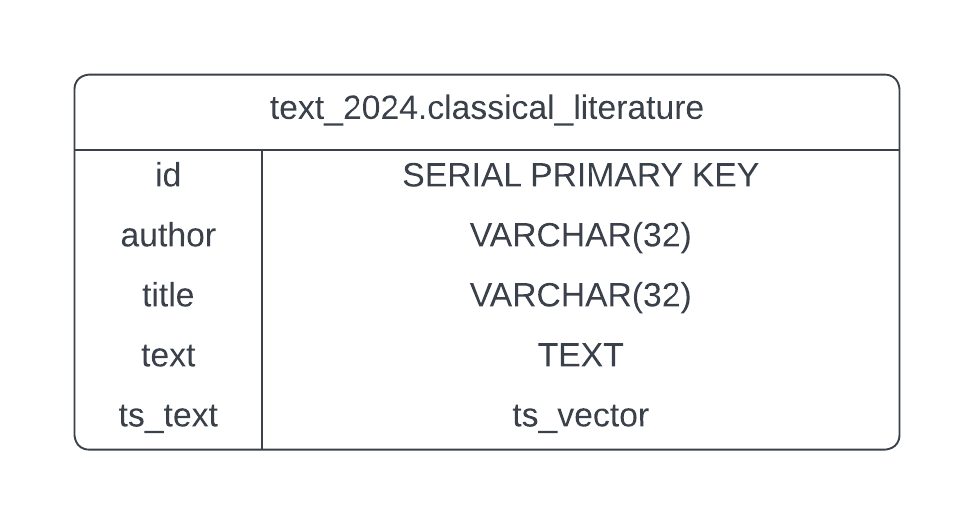
\includegraphics[width=\textwidth, scale=0.85]{figures/er-diagram}
    \caption{Схема базы данных}
    \label{schema}
\end{figure}

В листинге~\ref{init-db} продемонстрированы команды для создания таблицы.

\begin{algorithm}[H]
    \floatname{algorithm}{Листинг}
    \caption{Код SQL для создания таблицы}
    \label{init-db}
    \begin{lstlisting}[style=codelistingstyle]
      CREATE TABLE IF NOT EXISTS text_2024.classical_literature(
            id SERIAL,
            author character varying(32) NOT NULL,
            title character varying(32) NOT NULL,
            text TEXT NOT NULL
      );

      ALTER TABLE text_2024.classical_literature
            ADD CONSTRAINT pk_classical_literature PRIMARY KEY (id);

      ALTER TABLE text_2024.classical_literature ADD column ts_text tsvector;

      UPDATE text_2024.classical_literature
            SET ts_text = to_tsvector(
                  'russian',
                  text_2024.classical_literature.text
      );
      \end{lstlisting}
\end{algorithm}

\subsection{Подготовка текстовых данных}

Было отобрано 21 произведение классической литературы.
Тексты произведений взяты из открытого банка ФИПИ\footnote{\href{https://ege.fipi.ru/bank/index.php?proj=B9ACA5BBB2E19E434CD6BEC25284C67F}{Дата обращения \DTMdate{2024-09-15}: Открытый банк ФИПИ заданий ЕГЭ по информатике}} по информатике (фильтр по заданию с кодификатором $4.6$ \enquote{Текстовый процессор}).
Информация об отобранных текстах представлена в таблице~\ref{text-data}.
Подсчет слов был произведен утилитой \texttt{wc}.

\begin{longtable}{|c|l|l|l|}
    \hline
    \textbf{№} & \textbf{Автор} & \textbf{Название} & \textbf{\# слов}   \\ \hline
    1  & Булгаков М.А.    & Собачье сердце                      & 26033  \\ \hline
    2  & Лермонтов М.Ю.   & Герой нашего времен                 & 43200  \\ \hline
    3  & Некрасов Н.А.    & Кому на Руси жить хорошо            & 31893  \\ \hline
    4  & Чехов А.П.       & Человек в футляре                   & 4142   \\ \hline
    5  & Бах Р.Д.         & Чайка по имени Ливингстон           & 8426   \\ \hline
    6  & Стругацкие       & Понедельник начинается в субботу    & 60779  \\ \hline
    7  & Булгаков М.А.    & Мастер и Маргарита                  & 118013 \\ \hline
    8  & Гоголь Н.В.      & Вечера на хуторе близ Диканьки      & 63657  \\ \hline
    9  & Грин А.С.        & Алые Паруса                         & 20502  \\ \hline
    10 & Киплинг Д.Р.     & Маугли                              & 49554  \\ \hline
    11 & Куприн А.И.      & Поединок                            & 68311  \\ \hline
    12 & Лермонтов М.Ю.   & Мцыри                               & 3380   \\ \hline
    13 & Платонов А.П.    & Юшка                                & 2300   \\ \hline
    14 & Пушкин А.С.      & Дубровский                          & 21564  \\ \hline
    15 & Пушкин А.С.      & Евгений Онегин                      & 22649  \\ \hline
    16 & Пушкин А.С.      & Капитанская дочка                   & 30287  \\ \hline
    17 & Толстой Л.Н.     & Анна Каренина                       & 280023 \\ \hline
    18 & Толстой Л.Н.     & Севастопольские рассказы            & 36539  \\ \hline
    19 & Хемингуэй Э.М.   & Прощай оружие                       & 79316  \\ \hline
    20 & Чехов А.П.       & Воры                                & 4996   \\ \hline
    21 & Грин А.С.        & Бегущая по волнам                   & 57994  \\ \hline
    \caption{Список авторов и произведений}
    \label{text-data}
\end{longtable}

Для упрощения загрузки текстовых данных в СУБД была проведена предварительная очистка текста от несущественной информации (комментарии автора, оглавление, служебная информация редакции и т.п.).
Кроме того, из текста удалены символы переноса строки.
То есть весь текст представляет собой последовательность слов и символов, расположенных в одной строке.
Также ковычки заменены на двойной знак~\texttt{'}.
Это сделано для упрощения загрузки текстовых данных в Docker-контейнер при помощи \texttt{bash}-скрипта, срабатываемого автоматически при инициализации.

\subsection{Docker}

Контейнеризация реализована следующим образом.
В файле \texttt{compose.yaml} содержится рецепт запуска двух сервисов:
\begin{itemize}
    \item Docker-образ с PostgreSQL;
    \item Docker-образ с pgadmin4.
\end{itemize}

\noindent Оба сервиса связываются друг c другом через \texttt{docker network}.
После запуска контейнеров командой \texttt{docker compose up}~\cite{DockerComposeDocs} пользователь получает доступ к базе данных через локальный сервер по адресу \texttt{localhost:5050}.

\subsection{Загрузка текстовых данных в таблицу}

Для загрузки подготовленных произведений в СУБД на удаленном сервере использован \texttt{python}-скрипт.
Для создания таблицы и ее наполнения в Docker-контейнере написан \texttt{bash}-скрипт, который автоматически срабатывает во время развертывания контейнеров.
Все использованные скрипты доступны в репозитории\footnote{\href{https://github.com/artem-burashnikov/postgresql-fulltext-search}{Дата обращения \DTMdate{2024-09-15}: https://github.com/artem-burashnikov/postgresql-fulltext-search}}.

% \subsection{Некоторые типичные ошибки}
% Здесь мы будем собирать основные ошибки, которые случаются при написании текстов.
% В интернетах тоже можно найти коллекции типич\-ных косяков%
% \footnote{\href{https://www.read.seas.harvard.edu/~kohler/latex.html}{https://www.read.seas.harvard.edu/\textasciitilde kohler/latex.html} (дата обращения: \DTMdate{2022-12-16}).}.

% Рекомендуется по-умол\-ча\-нию использовать красивые греческие бук\-вы $\sigma$  и $\phi$, а именно $\phi$ вместо $\varphi$.
% В данном шаблоне команды для этих букв переставлены местами по сравнению с ванильным \TeX'ом.

% Также, если работа пишется на русском языке, необходимо, чтобы работа была написана на \textit{грамотном} русском языке даже если автор из ближнего зарубежья%
% \footnote{Теоретически, возможен вариант написания текстов на английском языке, но это необходимо обсудить в первую очередь с научным руководителем.}.
% Это включает в себя:
% \begin{itemize}
%     \item разделы должны оформляться с помощью \verb=\section{...}=, а также \verb=\subsection= и т.~п.; не нужно пытаться нумеровать вручную;
%     \item точки после окончания предложений должны присутствовать;
%     \item пробелы после запятых и точек, в конце слова перед скобкой;
%     \item неразрывные пробелы там, где нужны пробелы, но переносить на другую строку нельзя, например \verb=т.~е.=, \verb=А.~Н.~Терехов=, \verb=что-то~\cite{?}=, \verb=что-то~\ref{?}=;
%     \item дефис там, где нужен дефис (обозначается с помощью одиночного \enquote{минуса} (англ. dash) на клавиатуре);
%     \item двойной дефис там, где он нужен; а именно  при указании проме\-жутка в цифрах: в 1900--1910 г.~г., стр. 150--154;
%     \item тире (т.~е. \verb=---=~--- тройной минус) на месте тире, а не что-то другое; в русском языке тире не может \enquote{съезжать} на новую строку, поэтому стоит использовать такой синтаксис: \verb=До~--- после=;
%     \item даты стоит писать везде одинаково; чтобы об этом не следить, можно пользоваться заклинанием \verb=\DTMdate{2022-12-16}=;
%     \item правильные кавычки должны набираться с помощью пакета \texttt{csquotes}: для основного языка в \texttt{polyglossia} стоит использовать команду \verb=\enquote{текст}=, для второго языка стоит использовать \verb=\foreignquote{язык}{текст}=; правильные кавычки в русской типографии~--- \verb=<<ёлочки>>=, ни в коем случае не \verb="скандинавские лапки"=;
%     \item все перечисления должны оформляться с помощью \verb=\enumerate= или \verb=\itemize=; пункты перечислений должны либо начинаться с заглавной буквы и заканчиваться точкой, либо начинаться со строчной и закачиваться точкой с запятой; последний пункт пере\-числений всегда заканчивается точкой.
%     \item Перед выкладыванием финальной версии необходимо просмотреть лог \LaTeX'a, и обратить внимание на сообщения вида \emph{Overfull \textbackslash hbox (1.29312pt too wide) in paragraph}. Обычно, это означает, что текст выползает за поля, и надо подсказать, как правильно разделять слова на слоги, чтобы перенос произошел автоматически.
%           Это делается, например, так: \verb=соломо\-волокуша=.
%     \item \emph{Обязательно используйте инструменты автоматической проверки правописания!}
%           Не посылайте текст даже научному руководителю на проверку, если не прогнали спеллчекер%
%           \footnote{Например, для браузера можно использовать плагин LanguageTool, для VS Code --- Code Spell Checker с расширением для русского (но он вроде не умеет пунктуацию, так что следите за запятыми).}%
%           , желательно, умеющий проверять пунктуацию~--- у научника куча времени уйдёт на комментарии вида \enquote{тут нужна запятая} и не останется сил посоветовать что-нибудь по делу.
%           А ещё научник будет шокирован уровнем грамотности современной молодёжи, впадёт в депрессию и не будет отвечать вам неделю.
% \end{itemize}

% \subsection{Листинги, картинка и прочий \enquote{не текст}}

% Различный \enquote{не текст} имеет свойство отображаться не там, где он написан в текстовом виде в \LaTeX{}, поэтому у него должна быть самодостаточ\-ная понятная подпись \verb=\caption{...}=, уникальная метка \verb=\label{...}=, чтобы на неё можно было бы ссылаться в тексте с помощью \verb=\ref{...}= (более того, ссылка из текста обязательна).
% Ниже Вы сможете увидеть таблицу \ref{time_cmp_obj_func}, на которую мы сослались буквально только что.

% \enquote{Не текста} может быть довольно много~--- чтобы не засорять корневую папку, хорошим решением будет складывать весь \enquote{не текст} в папку \texttt{figures}.
% Заклинание \verb=\includegraphics{}= уже знает этот путь и будет искать там файлы без указания папки.
% Команда \verb=\input{}= умеет ходит по путям, например \verb=\input{figures/my_awesome_table.tex}=.
% Кроме того, листинги кода можно подтягивать из файла с помощью команды \verb=\inputminted{file}=.

% %% Вставка кода с помощью listings
% % \begin{lstlisting}[caption={Название для листинга кода. Достаточно длинное, чтобы люди, которые смотрят картинку сразу после названия статьи (т.~е. все люди), смогли разобраться и понять к чему в статье листинги, картинки и прочий \enquote{не текст}.}, language=Caml, frame=single]
% %   let x = 5 in x + 1
% % \end{lstlisting}

% %% Вставка кода с помощью minted
% \begin{listing}
%     \caption{Название для листинга кода. Достаточно длинное, чтобы люди, которые смотрят картинку сразу после названия статьи (т.~е. все люди), смогли разобраться и понять к чему в статье листинги, картинки и прочий \enquote{не текст}.}
%     \begin{minted}[frame=single]{ocaml}
%     let x = 5 in x + 1
%   \end{minted}
% \end{listing}

% \subsubsection{Выделение куска листинга с помощью tikz}
% Это бывает полезно в текстах, а ещё чаще~--- в презентациях.
% Пример сделан на основе вопроса на \textsc{StackExchange}%
% \footnote{Вопрос про рамку вокруг листинга на StackExchange, \url{https://tex.stackexchange.com/questions/284311} (дата обращения: \DTMdate{2022-12-16}).}.
% Заодно тут показывается альтернативный minted пакет, lstlistings, если не хотите ставить Python и пакет pygments.
% В этом случае закомментируйте всё, что связано с minted, в matmex-diploma-custom.cls.
% И внимательно следите за тем, чтобы везде использовался либо только lstlistings, либо minted~--- смешивание их в одном документе приведёт к странным ошибкам.

% \begin{figure}
%     % TODO(Kakadu): Сделать \lstset глобально, чтобы не выписывать все опции листингов каждый раз
%     \begin{lstlisting}[ escapechar=!, keepspaces=true, extendedchars=\true, texcl=true
%                       , basicstyle=\ttfamily, commentstyle=\color{eclipseGreen}\ttfamily\itshape, language=c ]
% #include <stdio.h>
% #include <math.h>

% /** A comment in English */
% int main(void)
% {
%   double c = -1;
%   double z = 0;

%   // Это комментарий на русском языке
%   printf ("For c = %lf:\n", c);
%   for (int i = 0; i < 10; i++ ) {
%     printf( !\tikzmark{a}!"z %d = %lf\n"!\tikzmark{b}!, i, z);
%     z = pow(z, 2) + c;
%   }
% }
% \end{lstlisting}

%     \begin{tikzpicture}[use tikzmark]
%         \draw[fill=gray,opacity=0.1]
%         ([shift={(-3pt,2ex)}]pic cs:a)
%         rectangle
%         ([shift={(3pt,-0.65ex)}]pic cs:b);
%     \end{tikzpicture}
%     \caption{Пример листинга c помощью пакета \texttt{listings} и \textsc{TIKZ} декорации к нему, оформленные в окружении \texttt{figure}.
%         Обратите внимание, что рисунок отображается не там, где он в документе, а может \enquote{плавать}.}
% \end{figure}

% \subsection{Некоторые детали описания реализации}
% Описание реализации~--- очень важный раздел для будущих программных инженеров, т.е. почти для всех.
% Важно иметь всегда, даже если Вы написали прототип на коленке или немного скриптов.

% В процессе работы можно сделать огромное количество косяков, неполный список которых ниже.

% \begin{enumerate}
%     \item Реализация должна быть.
%           На публично доступную реализацию обязательна ссылка (в заключении, но можно продублировать тут).
%           Если код под \textsc{NDA}, то об этом, во-первых, должно быть сказано явно,
%           во-вторых, на защиту должны выно\-ситься другие результаты (например, архитектура), чтобы комис\-сия имела возможность оценить хоть что-то,
%           и, в третьих, должна быть справка от работодателя, что Вы правда что-то сделали.
%           \begin{itemize}
%               \item Рецензент обязан оценить код (о возможности должен побеспо\-коиться обучающийся).
%           \end{itemize}
%     \item Код реализации должен быть написан защищающимся целиком.
%           \begin{itemize}
%               \item Если проект групповой, то нужно явно выделить, какие части были модифицированы защищающимся.
%                     Например, в преды\-дущих разделах на картинке архитектуры нужно выделить цветом то, что Вы модифицировали.
%               \item Нельзя пускать в негрупповой проект коммиты от других людей, или людей не похожих на Вас.
%                     Например, в 2022 году защищающийся-парень делал коммиты от сценического псев\-донима, который намекает на женский \enquote{гендер}.
%                     (Нет, это не шутка.)
%                     На тот момент в российской культуре это выглядело странно.
%               \item Возможна ситуация, что вы используете конкретный ник в интернете уже лет пять, и желаете писать ВКР под этим ником на \GitHub{}.
%                     В принципе, это допустимо, но если Вы встретите преподавателя, который считает наоборот, то Вам придется грамотно отмазы\-ваться.
%                     В Вашу пользу могут сыграть те факты, что к нику на \GitHub{} у Вас приписаны настоящие имя и фамилия; что в репозитории у вас видна домашка за первый курс;
%                     и что Ваш преподаватель практики сможет подтвердить, что Вы уже несколько лет используете это ник; и т.п.
%           \end{itemize}
%     \item Если Вы получаете диплом о присвоении квалификации программиста, код должен соответствовать.
%           \begin{enumerate}
%               \item Не стоит выкладывать код одним коммитом.
%               \item Не стоит выкладывать код аккурат перед защитой.
%               \item Лучше хоть какие-то тесты, чем совсем без них.
%                     В идеале нужно предъявлять процент покрытия кода тестами.
%               \item Лучше сделать \textsc{CI}, а также \textsc{CD}, если оно уместно в Вашем проекте.
%               \item Не стоит демонстрировать на защите, что Вам даже не пришло в голову напустить на код линтеры и т.п.
%           \end{enumerate}
%     \item Если ваша реализация по сути является прохождением стандартного туториала,
%           например, по отделению картинок кружек от котиков с помощью машинного обучения, то необходимо срочно сообщить об этом руководителю практики/ВКР,
%           иначе Государственная Экзаменацион\-ная Комиссия \enquote{порвёт Вас как Тузик грелку}, поставит \enquote{единицу},
%           а все остальные Ваши сокурсники получат оценку выше.
%           (Это не шутка, а реальная история 2020 года.)
% \end{enumerate}

% \noindent Если Вам предстоит защищать учебную практику, а эти рекомендации видятся как более подходящие для защиты ВКР, то ... отмаза не засчиты\-вается, сразу учитесь делать нормально.

% % !TeX spellcheck = ru_RU
% !TEX root = vkr.tex

\section{Эксперимент}

\subsection{Характеристики оборудования}
Оборудование, на котором были поставлены описанные далее эксперименты, обладает следующими характеристиками:
\subsubsection*{OS and Kernel}
\begin{verbatim}
Operating System: Ubuntu 22.04.2 LTS
          Kernel: Linux 5.19.0-41-generic
\end{verbatim}

\subsubsection*{CPU}
\begin{verbatim}
Architecture:       x86_64
Model name:         AMD Ryzen 5 4500U with Radeon Graphics
Thread(s) per core: 1
Core(s) per socket: 6
Socket(s):          1
CPU max MHz:        2375,0000
CPU min MHz:        1400,0000
L1d cache:          192 KiB (6 instances)
L1i cache:          192 KiB (6 instances)
L2 cache:           3 MiB (6 instances)
L3 cache:           8 MiB (2 instances)
\end{verbatim}

\subsubsection*{GPU}
\begin{verbatim}
Device: [AMD/ATI] Renoir (rev c3)
Memory: 256M
\end{verbatim}

\subsubsection*{RAM}
\begin{verbatim}
Memory:      7304
Swap memory: 2047
Total:       9351 
\end{verbatim}

\subsection{Исследовательские вопросы}
Анализ поставленных задач позволил выдвинуть следующие гипотезы:
{\parindent0pt
    
    \subsubsection*{RQ1}
    \label{RQ1}
    Ожидается, что в параллельной версии алгоритма обхода в ширину производительность будет значительно превышать последовательную версию на сильно разреженных неориентированных графах, потому что в таких графах большинство вершин имеют небольшую степень, что позволит эффективно распределить работу между потоками и уменьшить накладные расходы на синхронизацию. Таким образом, параллельная версия должна продемонстрировать ощутимое ускорение.
}
{\parindent0pt
    \subsubsection*{RQ2}
    \label{RQ2}
    Предполагается существование оптимального количества потоков в параллельной версии алгоритма, которое приведет к наибольшему выигрышу в производительности за счет эффективного использования доступных ресурсов вычислительной системы.
}

\subsection{Использованные метрики}

Для исследования~\hyperref[RQ1]{RQ1} решено замерять ускорение (Speedup) параллельной версии алгоритма относительно последовательной со следующим набором контролируемых параметров:
\begin{itemize}
    \item количество вершин в графе;
    \item плотность графа;
    \item количество используемых потоков.
\end{itemize}

Для поиска оптимального значения, обозначенного в~\hyperref[RQ2]{RQ2}, будет проанализировано среднее время работы параллельной версии алгоритма на сильно разреженных графах с использованием разного количества потоков: 1, 2, 4, 8, 16.

Все замеры будут выполнены с использованием библиотеки для измерения производительности \texttt{BenchmarkDotNet}~\cite{benchTool}, разрабатываемой и поддерживаемой для платформы \texttt{.NET}.

\subsection{Набор данных}
Для фиксации исследуемых величин были выбраны 10 различных разреженных квадратных матриц из коллекции университета Флориды~\cite{matrixData}.
Плотные матрицы было решено генерировать из разреженных постепенным и аккуратным добавлением ребёр до тех пор, пока структура не станет обладать нужными характеристиками. При этом необходимо, чтобы матрица смежности графа заполнялась значениями меток равномерно по всей площади двумерной сетки, потому как случайная группировка ребёр вокруг определенного квадранта матрицы может привести к нежелательным последствиям из-за особенности внутреннего представления матриц в виде деревьев квадрантов.

Информация о выбранных данных представлена в таблице~\ref{table:sparse_matrices}. 
Для обозначения числа ненулевых элементов используется аббревиатура \textit{Nnz}. 

В ней приведено официальное название матрицы (синтетические матрицы имеют то же имя, что и их прародители, но с добавлением префикса \textit{S}), количество строк, количество ненулевых элементов, соотношение ненулевых элементов к числу всех возможных элементов.

\begin{table}[h]
\begin{center}
\caption{Разреженные матричные данные}
\label{table:sparse_matrices}
\rowcolors{2}{black!2}{black!10}
\scalebox{1.0}{
\begin{tabular}{|l|r|r|r|}
\hline
Матрица & Количество cтрок $R$ & Nnz $M$ & Nnz/$R^{2}$ \\
\hline
\hline
%wing             &    62,032      &   243,088    & 3.9 \\
%luxembourg\_osm  &   114,599      &   239,332    & 2.0 \\
%amazon0312       &   400,727      & 3,200,400    & 7.9 \\
%amazon-2008      &   735,323      & 5,158,388    & 7.0 \\
%web-Google       &   916,428      & 5,105,039    & 5.5 \\
%roadNet-PA       & 1,090,920      & 3,083,796    & 2.8 \\
%roadNet-TX       & 1,393,383      & 3,843,320    & 2.7 \\
%belgium\_osm     & 1,441,295      & 3,099,940    & 2.1 \\
%roadNet-CA       & 1,971,281      & 5,533,214    & 2.8 \\
%netherlands\_osm & 2,216,688      & 4,882,476    & 2.2 \\ 
\hline
\end{tabular}
}
\end{center}
\end{table}


\subsection{Постановка эксперимента}
%Результаты понятно что такое. Тут всякие таблицы и графики, как в таблице \ref{time_cmp_obj_func}. Обратите внимание, как цифры выровнены по правому краю, названия по центру, а разделители $\times$ и $\pm$ друг под другом.

%Скорее всего Ваши измерения будут удовлетворять нормальному распределению, в идеале это надо проверять с помощью критерия Кол\-могорова и т.п.
%Если критерий этого не подтверждает, то у Вас что-то сильно не так с измерениями, надо проверять кэши процессора, отключать Интернет во время измерений, подкручивать среду исполне\-ния (англ. runtime), что\-бы сборка мусора не вмешивалась и т.п.
%Если критерий удовлетворён, то необходимо либо указать мат. ожидание и доверительный/предсказы\-вающий интервал, либо написать, что все измерения проводились с погрешностью, например, в 5\%.
%Замечание: если у вас получится улуч\-шение производительности в пределах погреш\-ности, то это обязательно вызовет вопросы.

%В этом разделе надо также коснуться Research Questions.

%\subsubsection{RQ1} Пояснения
%\subsubsection{RQ2} Пояснения

%\begin{table}
%\def\arraystretch{1.1}  % Растяжение строк в таблицах
%\setlength\tabcolsep{0.2em}
%\centering
% \resizebox{\linewidth}{!}{%
%    \caption{Производительность какого-то алгоритма при различных разрешениях картинок  (меньше~--- лучше), в мс.,  CI=0.95. За пример таблички кидаем чепчики в честь Я.~Кириленко}
%    \begin{tabular}[C]{
%    S[table-format=4.4,output-decimal-marker=\times]
%    *4{S
%          [table-figures-uncertainty=2, separate-uncertainty=true, table-align-uncertainty=true,
%          table-figures-integer=3, table-figures-decimal=2, round-precision=2,
%          table-number-alignment=center]
%          }
%    }
%    \toprule
%        \multicolumn{1}{r}{Resolution} & \multicolumn{1}{r}{\textsc{TENG}} & \multicolumn{1}{r}{\textsc{LAPM}} &
%        \multicolumn{1}{r}{\textsc{VOLL4}} \\ \midrule
%        1920.1080 & 406.23 \pm 0.94 & 134.06 \pm 0.35 & 207.45 \pm 0.42  \\ \midrule
%        1024.768  & 145.0 \pm 0.47  & 39.68 \pm 0.1   &  52.79  \pm 0.1 \\ \midrule
%        464.848   & 70.57 \pm 0.2   & 19.86 \pm 0.01 %    & 32.75  \pm 0.04 \\ \midrule
%        640.480   & 51.10 \pm 0.2   & 14.70 \pm 0.1 & 24  \pm 0.04 \\ \midrule
%        160.120   & 2.4 \pm 0.02    & 0.67 \pm 0.01      & 0.92  \pm 0.01 \\
%        \bottomrule
%    \end{tabular}%
%}
%    \label{time_cmp_obj_func}
%\end{table}

%\clearpage
%% !TeX spellcheck = ru_RU
% !TEX root = vkr.tex

\newcolumntype{C}{ >{\centering\arraybackslash} m{4cm} }
\newcommand\myvert[1]{\rotatebox[origin=c]{90}{#1}}
\newcommand\myvertcell[1]{\multirowcell{5}{\myvert{#1}}}
\newcommand\myvertcelll[1]{\multirowcell{4}{\myvert{#1}}}
\newcommand\myvertcellN[2]{\multirowcell{#1}{\myvert{#2}}}


\afterpage{%
    \clearpage% Flush earlier floats (otherwise order might not be correct)
    \thispagestyle{empty}% empty page style (?)
    \begin{landscape}% Landscape page
        \centering % Center table

\begin{tabular}{|c|c|c|c|c|c|c|c|c|c|c|c|c|c|c|c|c|c|}\hline
%& \multicolumn{17}{c|}{} \\ \hline
\multirowcell{2}{Код модуля \\в составе \\ дисциплины,\\практики и т.п. }
  &\myvertcellN{2}{Трудоёмкость\quad}
  & \multicolumn{10}{c|}{\tiny{Контактная работа обучающихся с преподавателем}}
  & \multicolumn{5}{c|}{\tiny{Самостоятельная работа}}
  & \myvertcellN{2}{\tiny Объем активных и интерактивных\quad}
  \\ \cline{3-17}

&& \myvertcellN{2}{лекции\quad}
    &\myvertcellN{2}{семинары\quad}
    &\myvertcellN{2}{консультации\quad}
    &\myvertcellN{2}{\small практические  занятия\quad}
    &\myvertcellN{2}{\small лабораторные работы\quad}
    &\myvertcellN{2}{\small контрольные работы\quad}
    &\myvertcellN{2}{\small коллоквиумы\quad}
    &\myvertcellN{2}{\small текущий контроль\quad}
    &\myvertcellN{2}{\small промежуточная аттестация\quad}
    &\myvertcellN{2}{\small итоговая аттестация\quad}

    &\myvertcellN{2}{\tiny под руководством    преподавателя\quad}
    &\myvertcellN{2}{\tiny в присутствии     преподавателя\quad}
    &\myvertcellN{2}{\tiny с использованием    методических\quad}
    &\myvertcellN{2}{\small текущий контроль\quad}
    &\myvertcellN{2}{\makecell{\small промежуточная \\ аттестация}}
    &     \\
&& &&&&&&&&& &&&&&&\\
&& &&&&&&&&& &&&&&&\\
&& &&&&&&&&& &&&&&&\\
&&&&&&&&&&& &&&&&&\\
&&&&&&&&&&& &&&&&&\\
&&&&&&&&&&& &&&&&&\\ \hline
Семестр 3 & 2 &30  &&&&&&&&2   & &&&18 &&20 &10\\ \hline
          &   &2--42&&&&&&&&2--25& &&&1--1&&1--1&\\ \hline
Итого     & 2 &30  &&&&&&&&2   & &&&18 &&20 &10\\ \hline
\end{tabular}

        \captionof{table}{Если таблица очень большая, то можно её изобразить на отдельной портретной странице. Не забудьте подробное описание, чтобы содержимое таблицы можно было понять не читая весь текст.}
    \end{landscape}
    \clearpage% Flush page
}



\subsection{Анализ результатов}

%Чуть более неформальное обсуждение, то, что сделано. Например, почему метод работает лучше остальных? Или, что делать со случаями, когда метод классифицирует вход некорректно.

% !TeX spellcheck = ru_RU
% !TEX root = artem-burashnikov_parallel_bfs_experiments.tex

\section*{Заключение}
В рамках выполнения данной работы проведено экспериментальное исследование. Получены следующие результаты.
\begin{itemize}
    \item Реализована параллельная и последовательная версии алгоритма обхода в ширину с использованием абстрактных операций линейной алгебры над матрицами и векторами, представленными в памяти как деревья.
    \item Оценено влияние плотности и количества вершин графа на эффективность параллельной версии обхода в ширину. В частности, установлены те параметы, при которых параллельная версия оказывается лучше последовательной.
    \item Найдено оптимально значение количества потоков, позволяющее получить максимальное ускорение.
\end{itemize}

Продолжение исследование может включать оценку ускорения параллельной версии обхода в ширину без использования линейной алгебры и представления матрицы как Quadtree.
Также интерес представляет выявление зависимости связности графа и выбора стартовой вершины (или вершин) на итоговую производительность алгоритма.

\setmonofont{CMU Typewriter Text}
\bibliographystyle{ugost2008ls}
\bibliography{vkr}

\end{document}
